\providecommand{\expplaceholder}{\textbf{***}}

\section{Experiments}
\label{sec:experiments}

This section tests whether role-shared semantic coordination improves task
correctness, preserves useful concurrent execution, and limits event-driven
updates to invalidated work. Simulation compares the proposed method with
three matched baselines over static, dynamic, and event conditions. Failure
counts and mechanism ablations then localize the source of the differences.
Hardware trials provide a physical check of the same semantic-state update
sequence.

\begin{figure}[t!]
  \centering
  \setlength{\tabcolsep}{3pt}
  % Equal-height cells align both columns while preserving each PDF aspect ratio.
  \newcommand{\ganttpanel}[1]{%
    \parbox[c][.93in][c]{.485\columnwidth}{\centering
      \includegraphics[width=.485\columnwidth]{#1}}}
  % The trajectory PDFs are shorter than their paired Gantt charts; lower
  % them slightly so the three row pairs share a common lower edge.
  \newcommand{\ganttpanelleft}[1]{%
    \parbox[c][.93in][c]{.485\columnwidth}{\centering
      \raisebox{+0.15in}{\includegraphics[width=.485\columnwidth]{#1}}}}
  \newcommand{\ganttrlabel}[1]{%
    \llap{\raisebox{.46in}{\textbf{(#1)}\hspace{2pt}}}}
  % Compact semantic-role response strip for each event row.
  \definecolor{g4affline}{HTML}{3E8050}
  \definecolor{g4afffill}{HTML}{F2F8F3}
  \definecolor{g4verline}{HTML}{B56A16}
  \definecolor{g4verfill}{HTML}{FFF8ED}
  \definecolor{g4planline}{HTML}{356FA8}
  \definecolor{g4planfill}{HTML}{F1F6FB}
  \newcommand{\rolechip}[5]{%
    \node[draw=#1,fill=#2,rounded corners=1.5pt,line width=0.45pt,
      minimum width=.285\columnwidth,text width=.265\columnwidth,
      minimum height=.19in,inner xsep=1.2pt,inner ysep=.6pt,
      align=center,font=\sffamily\fontsize{4.9}{5.4}\selectfont]
      at (#5) {\textbf{#3}\\[-1.5pt]#4};}
  \begin{tabular}{@{}cc@{}}
    \ganttrlabel{a}\ganttpanelleft{figures/figure_gantt/a1.pdf} &
    \ganttpanel{figures/figure_gantt/a2.pdf} \\
    \multicolumn{2}{@{}c@{}}{%
      
\begin{tikzpicture}[baseline=(current bounding box.center),x=1in,y=1in]
        \rolechip{g4affline}{g4afffill}{Affordance}{grounding unchanged}{0,0}
        \rolechip{g4verline}{g4verfill}{Verification}{instruction inconsistency}{.99,0}
        \rolechip{g4planline}{g4planfill}{Planning}{replace affected branch}{1.98,0}
      \end{tikzpicture}} \\[-2pt]
    \noalign{\vspace{2pt}}
    \ganttrlabel{b}\ganttpanelleft{figures/figure_gantt/b1.pdf} &
    \ganttpanel{figures/figure_gantt/b2.pdf} \\
    \multicolumn{2}{@{}c@{}}{%
      
\begin{tikzpicture}[baseline=(current bounding box.center),x=1in,y=1in]
        \rolechip{g4affline}{g4afffill}{Affordance}{target location updated}{0,0}
        \rolechip{g4verline}{g4verfill}{Verification}{dependency invalidated}{.99,0}
        \rolechip{g4planline}{g4planfill}{Planning}{recover downstream branch}{1.98,0}
      \end{tikzpicture}} \\[-2pt]
    \noalign{\vspace{2pt}}
    \ganttrlabel{c}\ganttpanelleft{figures/figure_gantt/c1.pdf} &
    \ganttpanel{figures/figure_gantt/c2.pdf} \\
    \multicolumn{2}{@{}c@{}}{%
      
\begin{tikzpicture}[baseline=(current bounding box.center),x=1in,y=1in]
        \rolechip{g4affline}{g4afffill}{Affordance}{workspace feasible}{0,0}
        \rolechip{g4verline}{g4verfill}{Verification}{n1 failed}{.99,0}
        \rolechip{g4planline}{g4planfill}{Planning}{assign repair branch}{1.98,0}
      \end{tikzpicture}}
  \end{tabular}

  \vspace{2pt}
  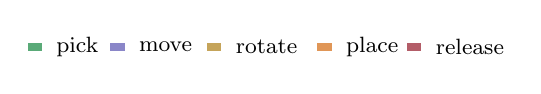
\begin{tikzpicture}[font=\rmfamily\fontsize{8}{8.8}\selectfont]
  \definecolor{gpick}{HTML}{5AAA78}
  \definecolor{gmove}{HTML}{8A86C8}
  \definecolor{grotate}{HTML}{C5A45A}
  \definecolor{gplace}{HTML}{E09657}
  \definecolor{grelease}{HTML}{B35D68}
  \foreach \x/\c/\t in {0/gpick/pick,1.05/gmove/move,2.28/grotate/rotate,
                          3.68/gplace/place,4.82/grelease/release}{
    \fill[\c] (\x,0) rectangle +(0.18,0.10);
    \node[anchor=west] at (\x+0.24,0.05) {\t};
  }
  \path[use as bounding box] (0,-0.08) rectangle (6.15,0.18);
\end{tikzpicture}


  \caption{Paired trajectories and execution timelines expose the localized
  response to each semantic event. (a) Task Update: the request changes to replace Mirinda with
  cola. (b) External Disturbance: the cola is moved to the other end of the
  conveyor during grasping. (c) Execution Failure: the conveyor moves too fast
  and both Franka manipulators fail their picks in succession. In each row,
  the left panel is the manipulator trajectory and the right panel is the
  corresponding Gantt chart.}
  \label{fig:gantt}
\end{figure}


\subsection{Experimental Setup}
\label{sec:experiment_setup}

The simulation uses the Isaac conveyor workspace in Fig.~\ref{fig:scenario}.
It contains heterogeneous manipulators, static and moving targets, global
visual observations, and a common primitive-skill interface. All methods use
the same scene and task assets, observations, success criterion, tracking and
safety stacks, and physical execution interface. Semantic calls use the LLM
\texttt{deepseek-ai/DeepSeek-V4-Flash} and the VLM
\texttt{Qwen/Qwen3.5-397B-A17B}. Conditions \texttt{C1}--\texttt{C4} cover
static and dynamic execution with task-relevant events \texttt{E1} (task
update), \texttt{E2} (external disturbance), and \texttt{E3} (verified
execution failure).
Each simulation condition contains 30 independent trials with randomly sampled
initial object layouts; events are injected at 30\%--70\% of subtask-completion
progress.
Evaluation uses task success, completion, efficiency, semantic reasoning, and
update-related metrics summarized in Tables~\ref{tab:baseline_tsr}--\ref{tab:hardware_results}
and the associated figures. Hardware conditions use 10 trials.

\subsection{Main Results}
\label{sec:main_results}

\begin{table}[t]
  \centering
  \caption{Baseline task success rate (TSR) over 30 trials across conditions.}
  \label{tab:baseline_tsr}
  \setlength{\tabcolsep}{2.0pt}
  \renewcommand{\arraystretch}{1.00}
  \scriptsize
  \begin{tabular*}{\columnwidth}{@{\extracolsep{\fill}}lcccccccc@{}}
    \toprule
    \multirow{2}{*}{\textbf{Method}} &
    \multirow{2}{*}{\textbf{C1}} &
    \multicolumn{3}{c}{\textbf{C2}} &
    \multirow{2}{*}{\textbf{C3}} &
    \multicolumn{3}{c}{\textbf{C4}} \\
    \cmidrule(lr){3-5}\cmidrule(lr){7-9}
    & & E1 & E2 & E3 & & E1 & E2 & E3 \\
    \midrule
    \textbf{Ours}
      & 30/30 & 30/30 & 30/30 & 30/30 & 27/30 & 30/30 & 30/30 & 27/30 \\
    End2End
      & 30/30 & 10/30 & 27/30 & 3/30 & 0/30 & 0/30 & 3/30 & 13/30 \\
    Agent per Robot
      & 10/30 & 3/30 & 13/30 & 17/30 & 3/30 & 0/30 & 0/30 & 0/30 \\
    COHERENT
      & 30/30 & 23/30 & 30/30 & 20/30 & 30/30 & 23/30 & 27/30 & 17/30 \\
    \bottomrule
  \end{tabular*}
\end{table}

\begin{figure}[!t]
  \centering
  \subfloat[SCR]{%
    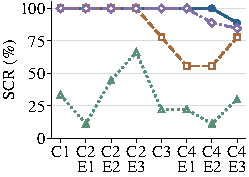
\includegraphics[width=.485\columnwidth]{figures/generated/figure5_a_scr.pdf}}
  \hfill
  \subfloat[Semantic reasoning time ratio]{%
    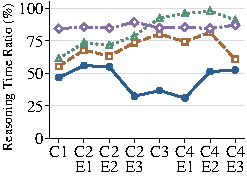
\includegraphics[width=.485\columnwidth]{figures/generated/figure5_b_reasoning_time.pdf}}
  \\[-1pt]
  \subfloat[Token usage]{%
    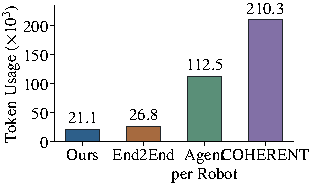
\includegraphics[width=.485\columnwidth]{figures/generated/figure5_c_token_usage.pdf}}
  \hfill
  \subfloat[Makespan]{%
    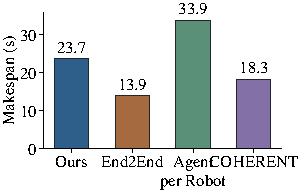
\includegraphics[width=.485\columnwidth]{figures/generated/figure5_d_makespan.pdf}}
  \\[-1pt]
  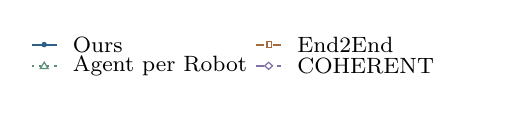
\begin{tikzpicture}[
    x=1cm,y=1cm,
    font=\rmfamily\fontsize{8}{8.8}\selectfont,
    legendline/.style={line width=.75pt}
  ]
    \definecolor{fours}{HTML}{2D5F8A}
    \definecolor{fend}{HTML}{A66A3F}
    \definecolor{fone}{HTML}{5A8F78}
    \definecolor{fcoh}{HTML}{8270A6}
    \draw[fours,legendline] (0,0)--(.32,0);
    \fill[fours] (.16,0) circle[radius=.035];
    \node[anchor=west] at (.40,0) {Ours};
    \draw[fend,legendline,dashed] (2.85,0)--(3.17,0);
    \draw[fend,line width=.45pt] (2.99,-.035) rectangle (3.05,.035);
    \node[anchor=west] at (3.25,0) {End2End};
    \draw[fone,legendline,dotted] (0,-.27)--(.32,-.27);
    \draw[fone,fill=white,line width=.45pt] (.16,-.225)--(.21,-.305)--(.11,-.305)--cycle;
    \node[anchor=west] at (.40,-.27) {Agent per Robot};
    \draw[fcoh,legendline,dash dot] (2.85,-.27)--(3.17,-.27);
    \draw[fcoh,fill=white,line width=.45pt]
      (3.01,-.225)--(3.06,-.27)--(3.01,-.315)--(2.96,-.27)--cycle;
    \node[anchor=west] at (3.25,-.27) {COHERENT};
    \path[use as bounding box] (-.05,-.38) rectangle (5.95,.12);
  \end{tikzpicture}
  \caption{Secondary event-handling metrics: (a) SCR, (b) semantic reasoning
  time ratio, (c) token usage, and (d) successful-trial makespan.}
  \label{fig:baseline_secondary}
\end{figure}



The proposed loop maintained high completion across all tested regimes while
changing only the event-relevant portion of the shared state. TSR was 30/30 in
the static, task-update, and disturbance conditions and 27/30 in the two
execution-failure conditions; SCR was 100\% except for 88.9\% in
\texttt{C4-E3}. The unsuccessful trials therefore occurred only under verified
execution-failure conditions rather than ordinary motion or task updates.
Figure~\ref{fig:event_graph_update} tracks the corresponding semantic-state
transitions. A task update revises $\gamma$ and the affected branches of $G$;
an external disturbance refreshes $\mathcal{F}$ and reconstructs branches whose
stored assumptions no longer hold; and an execution failure recorded in $z$
triggers repair of the failed node and its unfinished dependencies. In each
case, $\mathcal{N}_k^{\mathrm{aff}}$ is identified, unaffected valid nodes are
retained, and only the affected subgraph is reconstructed, providing
qualitative evidence of selective update.

The paired trajectories and timelines in Fig.~\ref{fig:gantt} show how this
design is realized. Verified independent nodes are dispatched together, local
tracking handles continuous target motion, and semantic reasoning is invoked
only at initialization, verification boundaries, or task-relevant events. The
reported time, makespan, and token ranges quantify this trade-off; the larger
token cost in \texttt{C4-E3} is consistent with its additional verified repair
branch.

\subsection{Comparison with Baselines}
\label{sec:baseline_comparison}

The comparison uses the same task, observations, capabilities, primitive
skills, trial count, and success criterion for every method. \textbf{End2End} directly
maps the task and observation to commands without the shared semantic state.
\textbf{Agent per Robot} gives each manipulator an independent language-model agent,
whereas \textbf{COHERENT} adapts the heterogeneous multi-robot collaboration protocol
of Liu~\emph{et al.}~\cite{liu2025coherent} to the same interface.

\begin{figure}[!t]
  \centering
  \newcommand{\failurePanel}[3]{%
  \begin{minipage}[t]{.485\columnwidth}
    \centering
    \includegraphics[width=\linewidth]{#1}
    \vspace{0.10em}
    {\scriptsize\textbf{(#2) #3}\par}
  \end{minipage}}

\failurePanel{figures/figure6/a.pdf}{a}{Invalid capability}
\hfill
\failurePanel{figures/figure6/b.pdf}{b}{Execution anomaly}
\vspace{0.35em}

\failurePanel{figures/figure6/c.pdf}{c}{Assignment conflict}
\hfill
\failurePanel{figures/figure6/d.pdf}{d}{Task timeout}

  \caption{Representative failures: (a) invalid workspace capability, (b)
  collision, (c) conflicting assignment, and (d) timeout after repeated
  replanning.}
  \label{fig:failure_analysis}
\end{figure}

\begin{figure}[!t]
  \centering
  % Generated PDF source:
% figures/generate_figure6_failure_distribution.py reads tables/failure.xlsx.
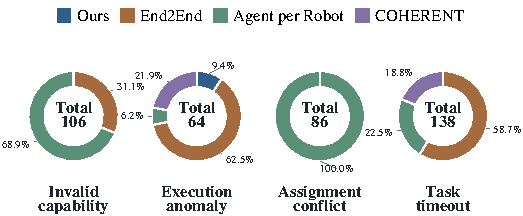
\includegraphics[width=\columnwidth]{figures/generated/figure6_e_failure_distribution.pdf}

  \vspace{-0.1in}
  \caption{Failure counts and baseline proportions by failure type.}
  \label{fig:failure_distribution}
\end{figure}


Ours retained 30/30 on all task-update
and disturbance cases and 27/30 under execution failure, while every baseline
lost substantially more event trials.
Table~\ref{tab:baseline_tsr} reports their
condition-wise TSR, making the event-specific gap below directly comparable.
The largest gap occurred when semantic events had to be incorporated.
In static \texttt{C1}, all methods except
Agent per Robot obtained 30/30, isolating the difference to event-aware
coordination rather than the basic skill interface.
The secondary metrics in Fig.~\ref{fig:baseline_secondary} show the same
ordering: among the compared methods, Ours had the highest event-condition SCR
and the lowest semantic-time ratio and token use. Ours had a longer
successful-trial makespan than End2End but higher event-condition completion.


\begin{figure*}[!t]
  \centering
  \newcommand{\figsevenframe}[1]{%
  \includegraphics[width=.188\textwidth]{figures/figure8/#1.jpg}}

\setlength{\tabcolsep}{1.1pt}
\renewcommand{\arraystretch}{0.92}
\begin{tabular}{@{}l@{\hspace{.35em}}ccccc@{}}
  \multicolumn{6}{@{}l}{\footnotesize\textbf{(a)} \texttt{H1} Normal cooperative execution: observe $\rightarrow$ assign $\rightarrow$ execute $\rightarrow$ place}
  \\[-1pt]
  & \figsevenframe{a-1} & \figsevenframe{a-2} & \figsevenframe{a-3}
  & \figsevenframe{a-4} & \figsevenframe{a-5} \\
  \multicolumn{6}{@{}l}{\footnotesize\textbf{(b)} \texttt{H2} Task update adaptation: execute current plan $\rightarrow$ update $\gamma$ $\rightarrow$ revise affected branch $\rightarrow$ continue execution}
  \\[-1pt]
  & \figsevenframe{c-1} & \figsevenframe{c-2} & \figsevenframe{c-3}
  & \figsevenframe{c-4} & \figsevenframe{c-5} \\
  \multicolumn{6}{@{}l}{\footnotesize\textbf{(c)} \texttt{H3} External disturbance recovery: approach target $\rightarrow$ human disturbance $\rightarrow$ verify inconsistency $\rightarrow$ recover downstream pick}
  \\[-1pt]
  & \figsevenframe{b-1} & \figsevenframe{b-2} & \figsevenframe{b-3}
  & \figsevenframe{b-4} & \figsevenframe{b-5} \\
\end{tabular}

  \vspace{-0.1in}
  \caption{Hardware sequences provide verification evidence for normal motion,
  task update, and external disturbance.}
  \label{fig:hardware_experiments}
\end{figure*}

\subsection{Failure Analysis and Ablation Study}
\label{sec:failure_analysis}
\label{sec:ablation}

\subsubsection{Cause of Task Failures}


The failure counts in Fig.~\ref{fig:failure_distribution} quantify the
intermediate coordination state. Ours had no capability, assignment, or timeout
failures and only six physical execution anomalies, whereas the baselines
exhibited the corresponding semantic failures. Fig.~\ref{fig:failure_analysis}
shows representative cases: role ownership filters invalid dispatches and
verification exposes residual physical anomalies for repair.

\subsubsection{Key Ablations}

\begin{table}[t]
  \centering
  \caption{Ablation TSR, SCR and Reasoning Time under
  \texttt{C4} (30 trials).}
  \label{tab:ablation_comparison}
  \setlength{\tabcolsep}{1.25pt}
  \renewcommand{\arraystretch}{1.00}
  \scriptsize
  \begin{tabular*}{\columnwidth}{@{\extracolsep{\fill}}lccccccccc@{}}
    \toprule
    \multirow{2}{*}{\textbf{Method}} &
    \multicolumn{3}{c}{\textbf{E1}} &
    \multicolumn{3}{c}{\textbf{E2}} &
    \multicolumn{3}{c}{\textbf{E3}} \\
    \cmidrule(lr){2-4}\cmidrule(lr){5-7}\cmidrule(lr){8-10}
    & {\fontsize{6.3}{6.8}\selectfont TSR}
    & {\fontsize{6.3}{6.8}\selectfont SCR}
    & {\fontsize{6.3}{6.8}\selectfont Time}
    & {\fontsize{6.3}{6.8}\selectfont TSR}
    & {\fontsize{6.3}{6.8}\selectfont SCR}
    & {\fontsize{6.3}{6.8}\selectfont Time}
    & {\fontsize{6.3}{6.8}\selectfont TSR}
    & {\fontsize{6.3}{6.8}\selectfont SCR}
    & {\fontsize{6.3}{6.8}\selectfont Time} \\
    \midrule
    \textbf{Ours}
      & \textbf{30/30} & \textbf{100} & \textbf{.309}
      & \textbf{30/30} & \textbf{100} & \textbf{.513}
      & \textbf{27/30} & 88.9 & \textbf{.525} \\
    \shortstack[l]{w/o Role\\Separation}
      & 23/30 & 82.1 & .462
      & \textbf{30/30} & \textbf{100} & .567
      & 0/30 & 78.2 & .796 \\
    \shortstack[l]{w/o Selective\\Replanning}
      & 26/30 & \textbf{100} & .456
      & \textbf{30/30} & \textbf{100} & .545
      & 17/30 & \textbf{93.0} & .658 \\
    \bottomrule
  \end{tabular*}
\end{table}


\begin{figure}[!t]
  \centering
  % Generated PDF source:
% The generator reads tables/failure.xlsx and produces the manuscript's Figure 8.
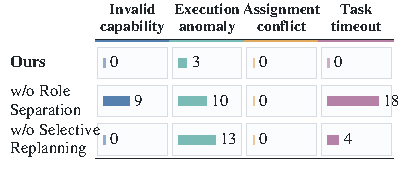
\includegraphics[width=\columnwidth]{figures/generated/figure7_ablation_failure_count.pdf}

  \vspace{-0.1in}
  \caption{Ablation failure counts under \texttt{C4}. A1 and A2 denote the
  variants without role separation and selective replanning, respectively.}
  \label{fig:ablation_failure_count}
\end{figure}


\begin{table}[t]
  \centering
  \caption{Hardware results over 10 trials. Resp. is event-response time (s);
  Aff./Pend. is the affected-to-pending node ratio.}
  \label{tab:hardware_results}
  \small
  \setlength{\tabcolsep}{2.8pt}
  \begin{tabular}{lcccc}
    \toprule
    Condition & TSR & SCR (\%) & Resp. (s) & Aff./Pend. \\
    \midrule
    \texttt{H1} Normal
      & 10/10 & 100.0 & --   & --   \\
    \texttt{H2} Task Update
      & 9/10  & 98.6  & 11.3 & 0.38 \\
    \texttt{H3} External Disturbance
      & 7/10  & 92.3  & 9.7  & 0.14 \\
    \bottomrule
  \end{tabular}
\end{table}

\begin{figure}[t]
  \centering
  \setlength{\tabcolsep}{.5pt}
  \begin{tabular}{@{}lccc@{}}
    \raisebox{8pt}{%
      \shortstack[r]{%
        \fontsize{8}{9}\selectfont L. Franka\\[3pt]
        \fontsize{8}{9}\selectfont R. Franka\\[3pt]
        \fontsize{8}{9}\selectfont Ranger}} &
    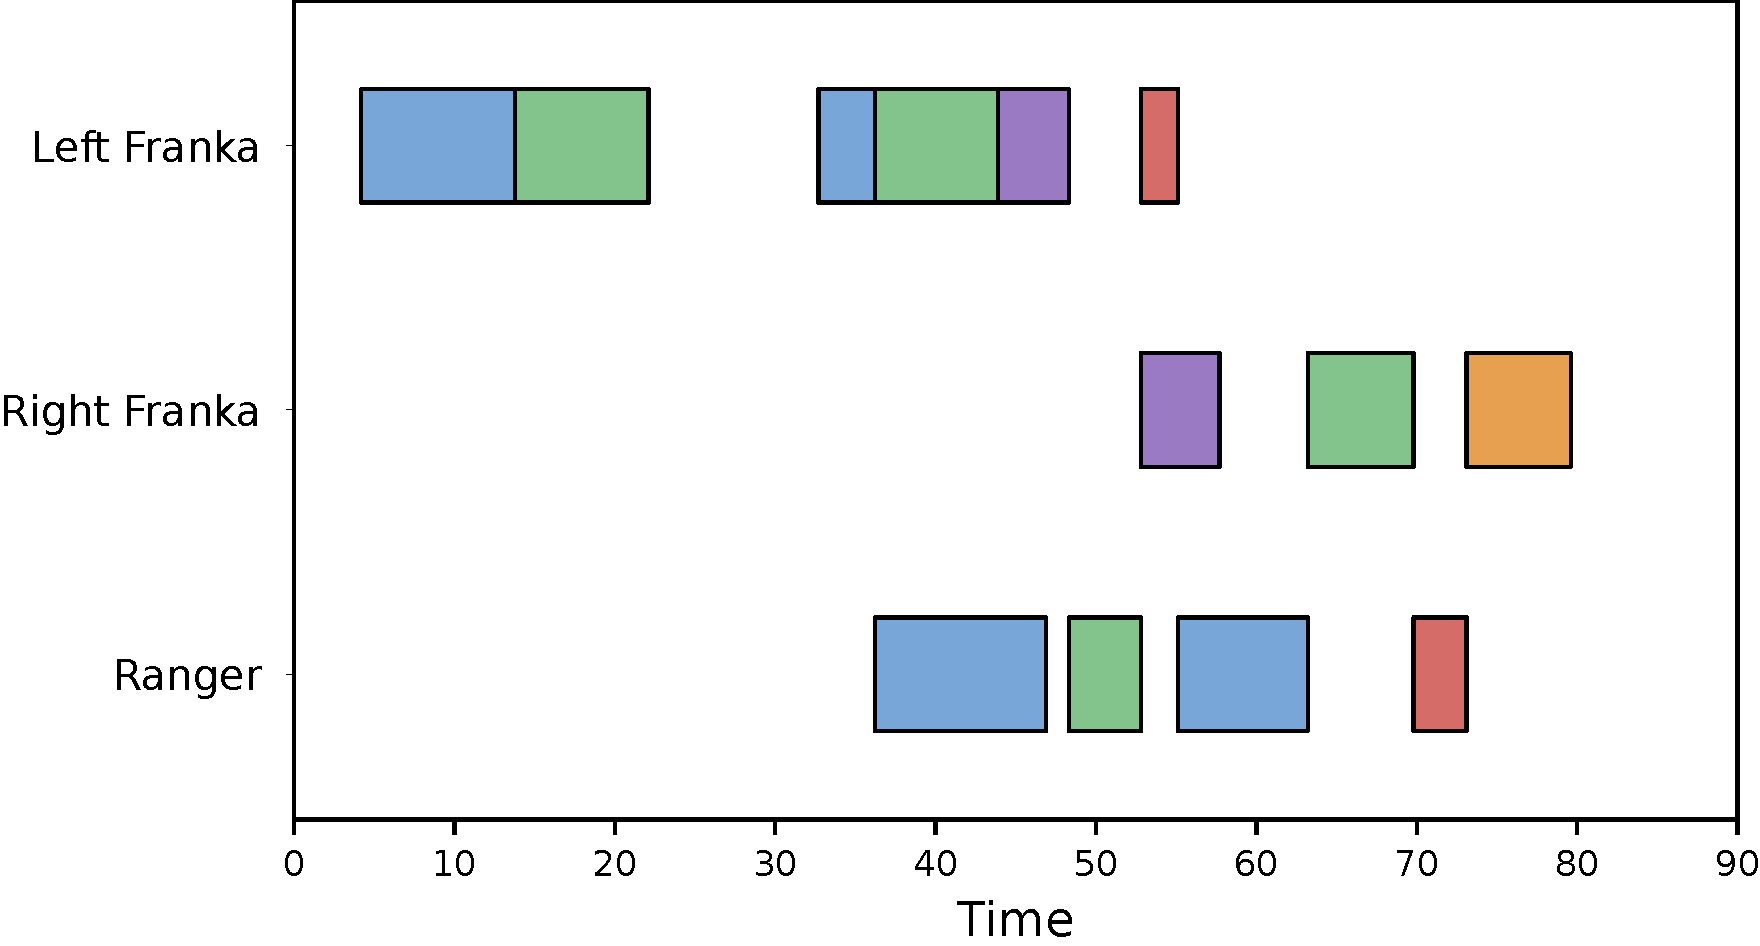
\includegraphics[trim=126pt 28pt 0 0,clip,width=.27\columnwidth]{figures/figure_new/a.pdf} &
    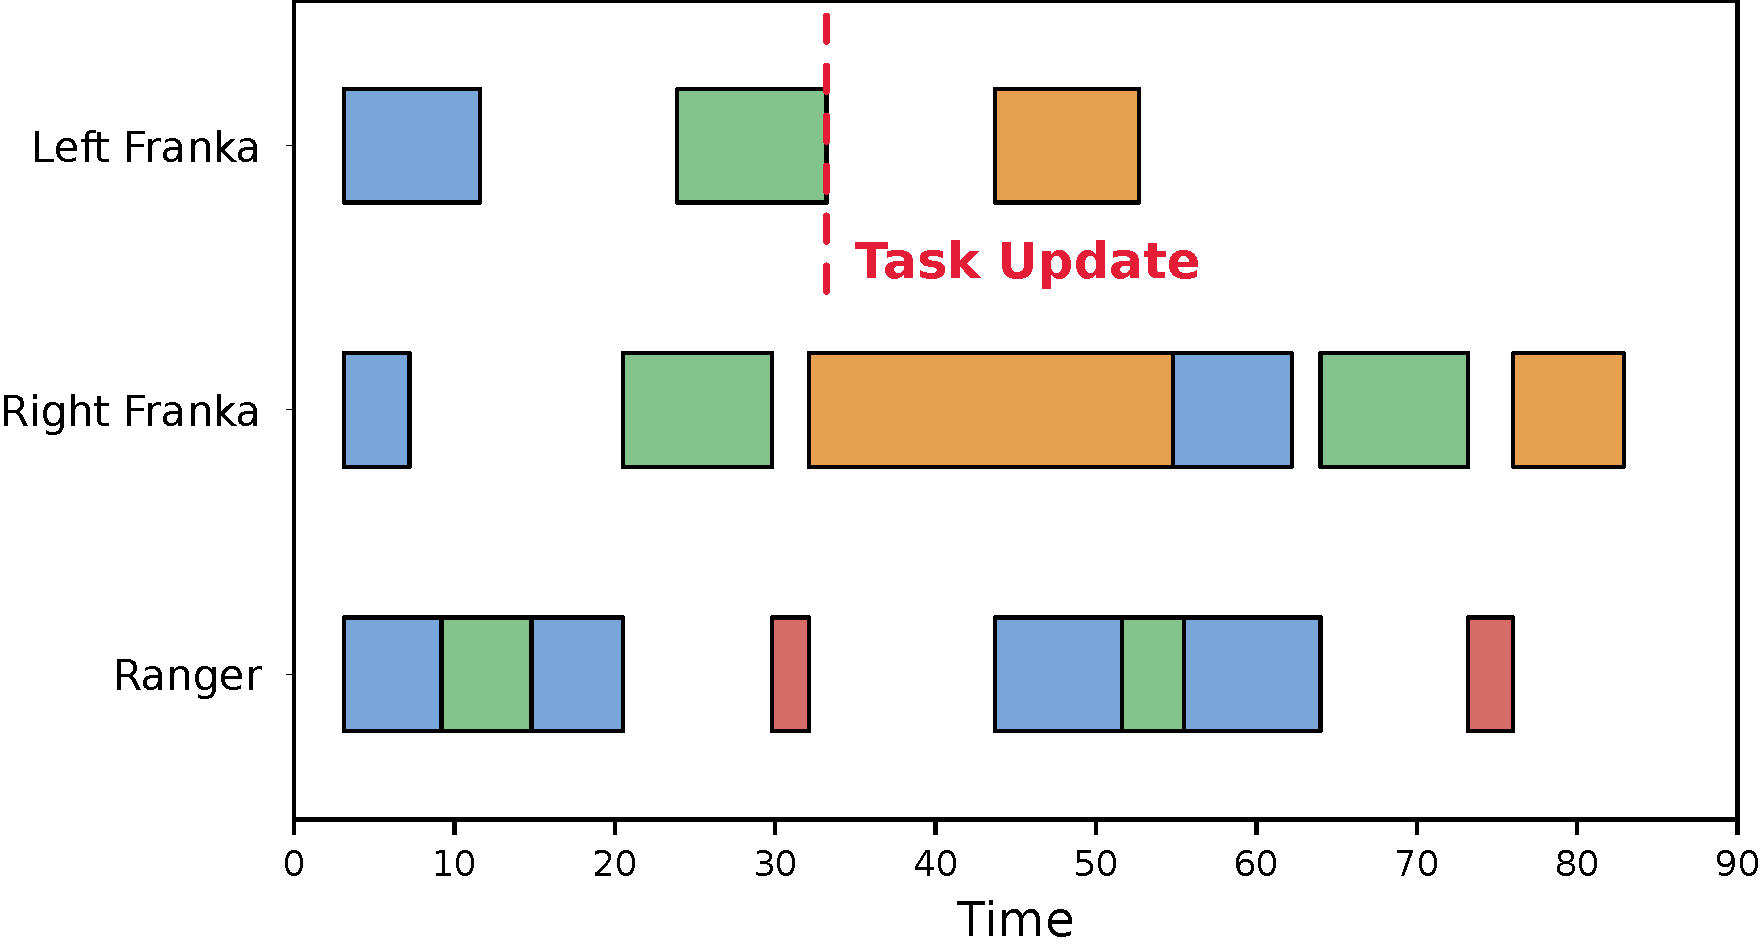
\includegraphics[trim=126pt 28pt 0 0,clip,width=.27\columnwidth]{figures/figure_new/b.pdf} &
    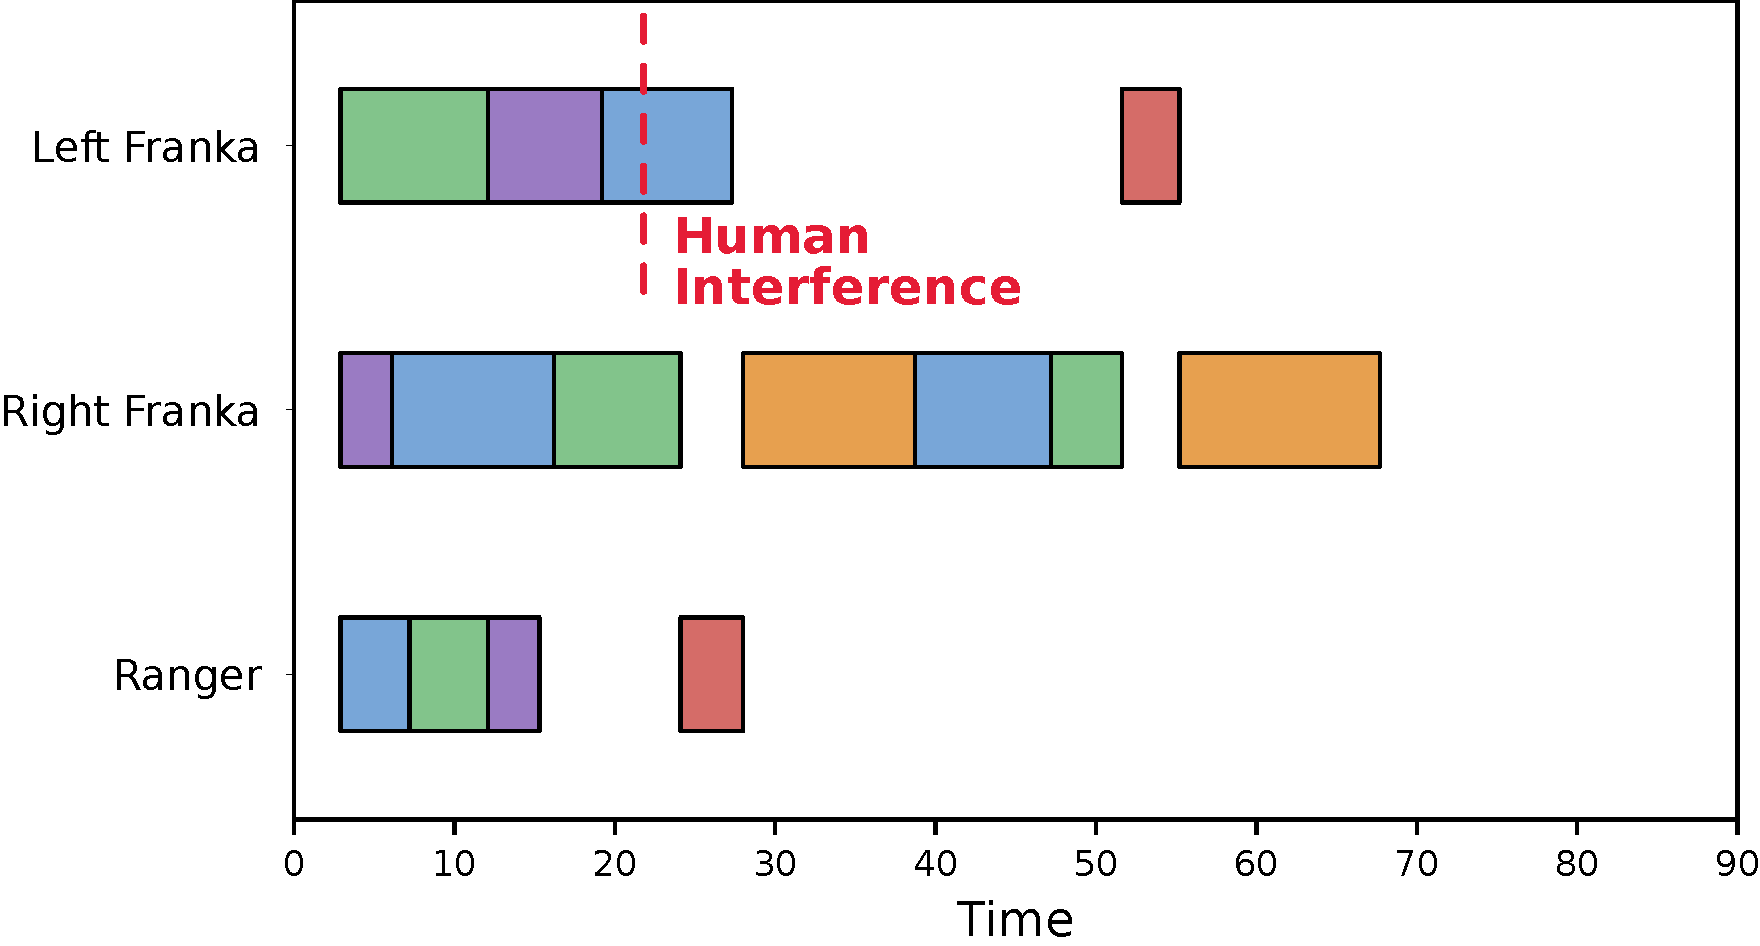
\includegraphics[trim=126pt 28pt 0 0,clip,width=.27\columnwidth]{figures/figure_new/c.pdf}
  \end{tabular}

  \vspace{1pt}
  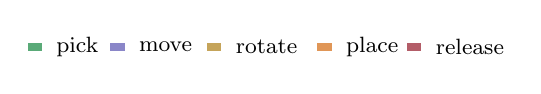
\begin{tikzpicture}[font=\rmfamily\fontsize{8}{8.8}\selectfont]
  \definecolor{gpick}{HTML}{5AAA78}
  \definecolor{gmove}{HTML}{8A86C8}
  \definecolor{grotate}{HTML}{C5A45A}
  \definecolor{gplace}{HTML}{E09657}
  \definecolor{grelease}{HTML}{B35D68}
  \foreach \x/\c/\t in {0/gpick/pick,1.05/gmove/move,2.28/grotate/rotate,
                          3.68/gplace/place,4.82/grelease/release}{
    \fill[\c] (\x,0) rectangle +(0.18,0.10);
    \node[anchor=west] at (\x+0.24,0.05) {\t};
  }
  \path[use as bounding box] (0,-0.08) rectangle (6.15,0.18);
\end{tikzpicture}

\vspace{-0.1in}
  \caption{Hardware timelines for Fig.~\ref{fig:hardware_experiments}: left,
  normal motion; middle, task-update revision; right, disturbance recovery.}
  \label{fig:hardware_gantt}
\end{figure}



Under \texttt{C4}, the ablations remove role ownership or selective replanning.
Table~\ref{tab:ablation_comparison} shows lower event TSR for both, most under
execution failure. Role-ablation errors in
Fig.~\ref{fig:ablation_failure_count} support this attribution: the
role-separated design limits error propagation by assigning each updated
semantic component a dedicated owner, namely affordance for $\mathcal{F}$,
planning for $G$, and verification for $z$. Without selective replanning,
higher semantic-time ratios show that semantic reasoning occupies more of the
execution horizon. Together with the lower event TSR, this result associates
selective replanning with lower semantic reasoning occupancy and better task
progress under the tested events.

\subsection{Hardware Experiments}
\label{sec:hardware_experiments}

The hardware platform contains two fixed Franka manipulators and a third
manipulator on an AgileX Ranger Mini V2. An AgileX SCOUT MINI carries task
objects as a teleoperated moving carrier; it is not a semantic coordinator.
The same shared state, primitive-skill interface, and event update path are
used on hardware. Each condition is repeated for 10 trials.
Figure~\ref{fig:hardware_role_outputs} exposes the role-level semantic updates
for the task-update and disturbance trials. In the top row, the revised
instruction enters $\gamma$, the affordance role refreshes $\mathcal{F}$, the
verification role identifies the affected nodes, and the planning role revises
$G$ while retaining unaffected work. The object relocation
refreshes $\mathcal{F}$, verification records the failed execution status in
$z$ and traces the invalidated dependencies, and planning repairs the affected
branch of $G$. The three role outputs are committed together as the
corresponding update of $S_{\mathrm{sem}}$ before dispatch resumes.




\begin{figure}[!t]
  \centering
  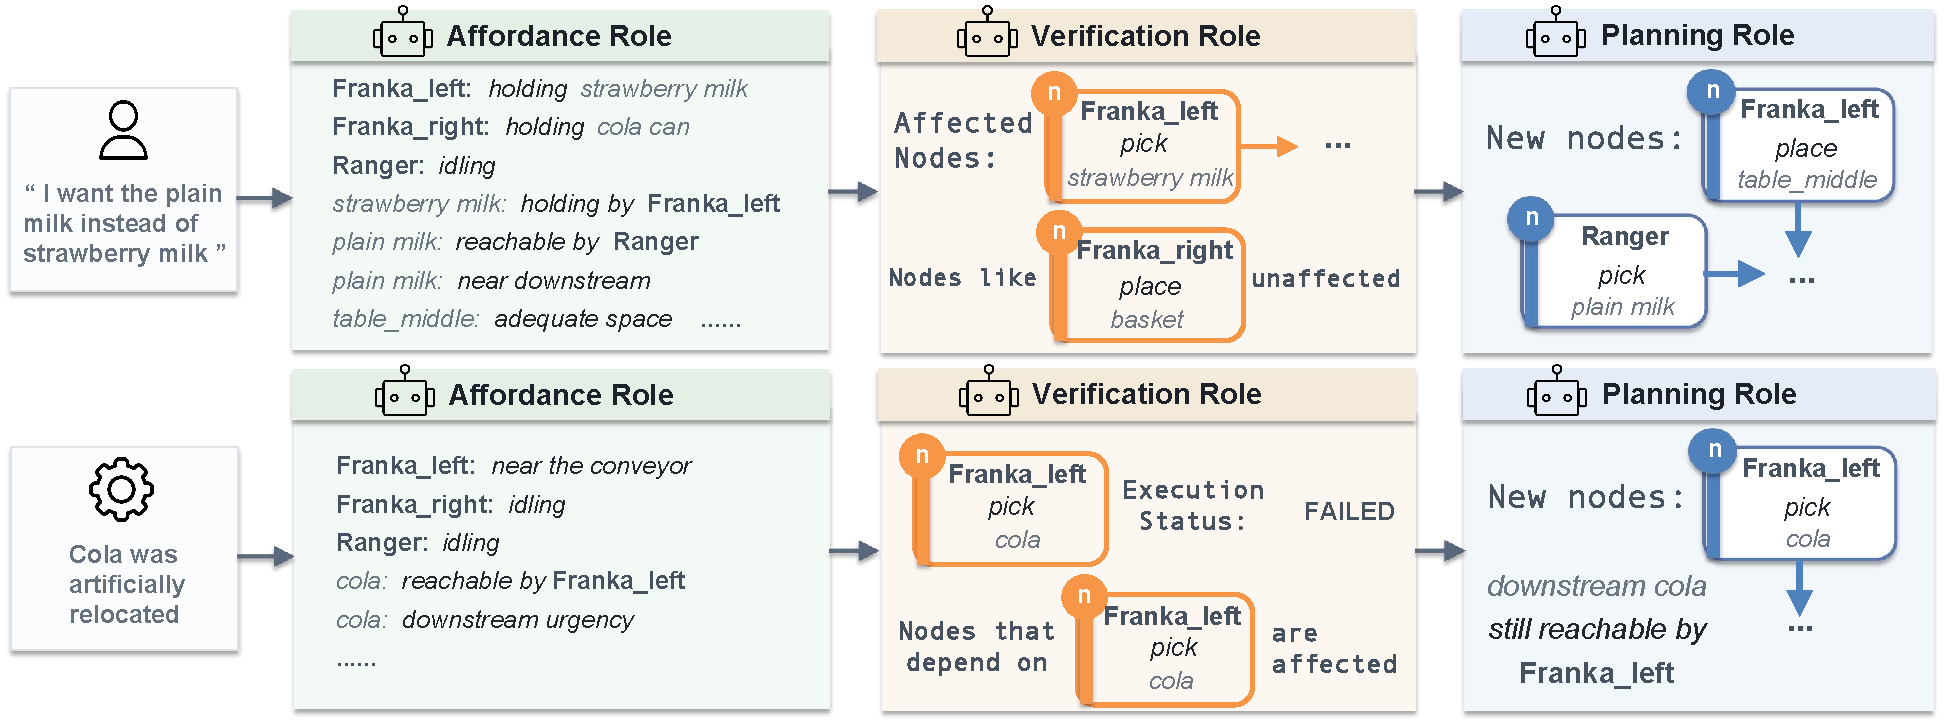
\includegraphics[width=\columnwidth]{figures/figure_role/figure_role.pdf}
  \caption{Intermediate outputs of the affordance, verification, and planning
  roles after the task-update event in the middle panel of
  Fig.~\ref{fig:hardware_gantt} (\textbf{Top}) and the external disturbance in the
  right panel (\textbf{Bottom}).}

  \label{fig:hardware_role_outputs}
\end{figure}


The three scenarios isolate normal motion, a task update, and a disturbance.
Table~\ref{tab:hardware_results} reports 10/10 TSR and 100.0\% SCR for
\texttt{H1}, 9/10 and 98.6\% for \texttt{H2} (11.3 s response, 0.38
affected/pending), and 7/10 and 92.3\% for \texttt{H3} (9.7 s, 0.14).
The recorded traces show that semantic updates are committed online before
dispatch resumes rather than reconstructed after a run: H2 updates $\gamma$
after the instruction change, H3 refreshes $\mathcal{F}$ after the disturbance,
and verification updates $z$ at execution boundaries. In H3, the resulting
revision covers a 14\% affected scope while retaining unaffected work. These
physical executions therefore corroborate the online update sequence; the
lower H3 TSR also shows that selective updating does not eliminate physical
uncertainty.
